\section{Smlar}

Поиск похожести в больших базах данных является важным вопросом в настоящее время для таких систем как блоги (похожие статьи), интернет-магазины (похожие продукты), хостинг изображений (похожие изображения, поиск дубликатов изображений) и т.д. PostgreSQL позволяет сделать такой поиск более легким. Прежде всего необходимо понять, как мы будем вычислять сходство двух объектов.

\subsection{Похожесть}

Любой объект может быть описан как список характеристик. Например, статья в блоге может быть описана тегами, продукт в интернет-магазине может быть описан размером, весом, цветом и т.д. Это означает, что для каждого объекта можно создать цифровую подпись~--- массив чисел, описывающих объект (\href{http://en.wikipedia.org/wiki/Fingerprint}{отпечатки пальцев}, \href{http://en.wikipedia.org/wiki/N-gram}{n-grams}). То есть нужно создать массив из цифр для описания каждого объекта.

\subsection{Расчет похожести}

Есть несколько методов вычисления похожести сигнатур объектов. Прежде всего, легенда для расчетов:

\begin{itemize}
  \item $N_a$, $N_b$~--- количество уникальных элементов в массивах;
  \item $N_u$~--- количество уникальных элементов при объединении массивов;
  \item $N_i$~--- количество уникальных элементов при пересечении массивов.
\end{itemize}

Один из простейших расчетов похожести двух объектов - количество уникальных элементов при пересечении массивов делить на количество уникальных элементов в двух массивах:

\begin{equation}
 \label{eq:smlar1}
 S(A,B) = \frac{N_{i}}{(N_{a}+N_{b})}
\end{equation}

или проще

\begin{equation}
 \label{eq:smlar2}
 S(A,B) = \frac{N_{i}}{N_{u}}
\end{equation}

Преимущества:

\begin{itemize}
  \item Легко понять;
  \item Скорость расчета: $N * \log{N}$;
  \item Хорошо работает на похожих и больших $N_a$ и $N_b$;
\end{itemize}

Также похожесть можно рассчитать по \href{http://en.wikipedia.org/wiki/Law\_of\_cosines}{формуле косинусов}:

\begin{equation}
 \label{eq:smlar3}
 S(A,B) = \frac{N_{i}}{\sqrt{N_{a}*N_{b}}}
\end{equation}

Преимущества:

\begin{itemize}
  \item Скорость расчета: $N * \log{N}$;
  \item Отлично работает на больших $N$;
\end{itemize}

Но у обоих этих методов есть общие проблемы:

\begin{itemize}
  \item Если элементов мало, то разброс похожести не велик;
  \item Глобальная статистика: частые элементы ведут к тому, что вес ниже;
  \item Спамеры и недобросовестные пользователи могут разрушить работу алгоритма и он перестанет работать на Вас;
\end{itemize}

Для избежания этих проблем можно воспользоваться \href{http://en.wikipedia.org/wiki/Tf*idf}{TF/IDF метрикой}:

\begin{equation}
 \label{eq:smlar4}
 S(A,B) = \frac{\sum_{i < N_{a}, j < N_{b}, A_{i} = B_{j}}TF_{i} * TF_{j}}{\sqrt{\sum_{i < N_{a}}TF_{i}^{2} * \sum_{j < N_{b}}TF_{j}^{2}}}
\end{equation}

где инвертированный вес элемента в коллекции:

\begin{equation}
 \label{eq:smlar5}
 IDF_{element} = \log{(\frac{N_{objects}}{N_{objects\ with\ element}} + 1)}
\end{equation}

и вес элемента в массиве:

\begin{equation}
 \label{eq:smlar6}
 TF_{element} = IDF_{element} * N_{occurrences}
\end{equation}

Все эти алгоритмы встроены в smlar расширение. Главное понимать, что для TF/IDF метрики требуется вспомогательная таблица для хранения данных, по сравнению с другими простыми метриками.

\subsection{Smlar}

Олег Бартунов и Теодор Сигаев разработали PostgreSQL расширение \href{http://sigaev.ru/git/gitweb.cgi?p=smlar.git;a=blob;hb=HEAD;f=README}{smlar}, которое предоставляет несколько методов для расчета похожести массивов (все встроенные типы данных поддерживаются) и оператор для расчета похожести с поддержкой индекса на базе GIST и GIN. Для начала установим это расширение:

\begin{lstlisting}[language=Bash,label=lst:smlar1,caption=Установка smlar]
$ git clone git://sigaev.ru/smlar
$ cd smlar
$ USE_PGXS=1 make && make install
\end{lstlisting}

Теперь проверим расширение:

\begin{lstlisting}[language=SQL,label=lst:smlar4,caption=Проверка smlar]
$ psql
psql (9.5.1)
Type "help" for help.

test=# CREATE EXTENSION smlar;
CREATE EXTENSION

test=# SELECT smlar('{1,4,6}'::int[], '{5,4,6}'::int[]);
  smlar
----------
 0.666667
(1 row)

test=# SELECT smlar('{1,4,6}'::int[], '{5,4,6}'::int[], 'N.i / sqrt(N.a * N.b)' );
  smlar
----------
 0.666667
(1 row)
\end{lstlisting}

Методы, которые предоставляет это расширение:

\begin{itemize}
  \item \lstinline!float4 smlar(anyarray, anyarray)!~--- вычисляет похожесть двух массивов. Массивы должны быть одного типа;
  \item \lstinline!float4 smlar(anyarray, anyarray, bool useIntersect)!~--- вычисляет похожесть двух массивов составных типов. Составной тип выглядит следующим образом:

\begin{lstlisting}[label=lst:smlar5,caption=Составной тип]
CREATE TYPE type_name AS (element_name anytype, weight_name float4);
\end{lstlisting}

  \lstinline!useIntersect! параметр для использования пересекающихся элементов в знаменателе;
  \item \lstinline!float4 smlar( anyarray a, anyarray b, text formula )!~--- вычисляет похожесть двух массивов по данной формуле, массивы должны быть того же типа. Доступные переменные в формуле:

    \begin{itemize}
      \item N.i~--- количество общих элементов обоих массивов (пересечение);
      \item N.a~--- количество уникальных элементов первого массива;
      \item N.b~--- количество уникальных элементов второго массива;
    \end{itemize}

  \item \lstinline!anyarray % anyarray!~--- возвращает истину, если похожесть массивов больше, чем указанный предел. Предел указывается в конфиге PostgreSQL:

\begin{lstlisting}[label=lst:smlar6,caption=Smlar предел]
custom_variable_classes = 'smlar'
smlar.threshold = 0.8 # предел от 0 до 1
\end{lstlisting}

Также в конфиге можно указать дополнительные настройки для smlar:

\begin{lstlisting}[label=lst:smlar7,caption=Smlar настройки]
custom_variable_classes = 'smlar'
smlar.threshold = 0.8 # предел от 0 до 1
smlar.type = 'cosine' # по какой формуле производить расчет похожести: cosine, tfidf, overlap
smlar.stattable = 'stat' # Имя таблицы для хранения статистики при работе по формуле tfidf
\end{lstlisting}

Более подробно можно прочитать в README этого расширения.
\end{itemize}

GiST и GIN индексы поддерживаются для оператора \lstinline!%!.


\subsection{Пример: поиск дубликатов картинок}

Рассмотрим простой пример поиска дубликатов картинок. Алгоритм помогает найти похожие изображения, которые, например, незначительно отличаются (изображение обесцветили, добавили водяные знаки, пропустили через фильтры). Но, поскольку точность мала, то у алгоритма есть и позитивная сторона~--- скорость работы. Как можно определить, что картинки похожи? Самый простой метод~--- сравнивать попиксельно два изображения. Но скорость такой работы будет не велика на больших разрешениях. Тем более, такой метод не учитывает, что могли изменять уровень света, насыщенность и прочие характеристики изображения. Нам нужно создать сигнатуру для картинок в виде массива цифр:

\begin{figure}[ht!]
  \center{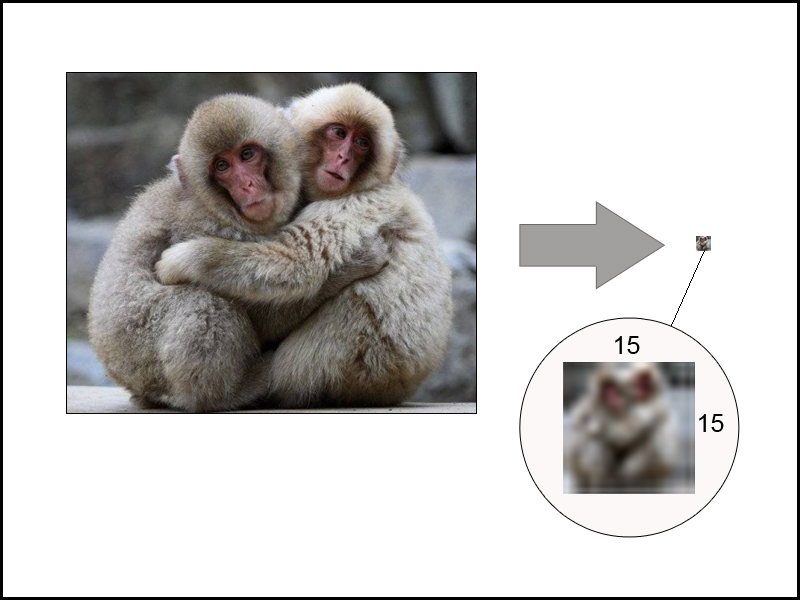
\includegraphics[width=1\textwidth]{smlar1.pdf}}
  \caption{Пиксельная матрица}
  \label{fig:smlar1}
\end{figure}

\begin{itemize}
  \item Создаем пиксельную матрицу к изображению (изменения размера изображения к требуемоему размеру пиксельной матрице), например 15X15 пикселей(Рис.~\ref{fig:smlar1});
  \item Рассчитаем интенсивность каждого пикселя (интенсивность вычисляется по формуле $0.299 * \textup{красный} + 0.587 * \textup{зеленый} + 0.114 * \textup{синий}$). Интенсивность поможет нам находить похожие изображения, не обращая внимание на используемые цвета в них;
  \item Узнаем отношение интенсивности каждого пикселя к среднему значению интенсивности по всей матрице(Рис.~\ref{fig:smlar2});
  \item Генерируем уникальное число для каждой ячейки (отношение интенсивности + координаты ячейки);
  \item Сигнатура для картинки готова;
\end{itemize}

\begin{figure}[ht!]
  \center{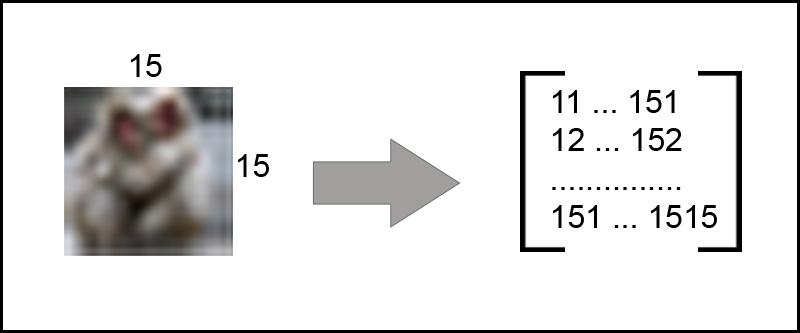
\includegraphics[width=1\textwidth]{smlar2.pdf}}
  \caption{Пиксельная матрица}
  \label{fig:smlar2}
\end{figure}

Создаем таблицу, где будем хранить имя картинки, путь к ней и её сигнатуру:

\begin{lstlisting}[language=SQL,label=lst:smlar8,caption=Таблица для изображений]
CREATE TABLE images (
 id serial PRIMARY KEY,
 name varchar(50),
 img_path varchar(250),
 image_array integer[]
);
\end{lstlisting}

Создадим GIN или GIST индекс:

\begin{lstlisting}[language=SQL,label=lst:smlar9,caption=Создание GIN или GIST индекса]
CREATE INDEX image_array_gin ON images USING GIN(image_array _int4_sml_ops);
CREATE INDEX image_array_gist ON images USING GIST(image_array _int4_sml_ops);
\end{lstlisting}

Теперь можно произвести поиск дубликатов:

\begin{lstlisting}[language=SQL,label=lst:smlar10,caption=Поиск дубликатов]
test=# SELECT count(*) from images;
  count
---------
 1000000
(1 row)

test=# EXPLAIN ANALYZE SELECT count(*) FROM images WHERE images.image_array % '{1010259,1011253,...,2423253,2424252}'::int[];

 Bitmap Heap Scan on images  (cost=286.64..3969.45 rows=986 width=4) (actual time=504.312..2047.533 rows=200000 loops=1)
   Recheck Cond: (image_array % '{1010259,1011253,...,2423253,2424252}'::integer[])
   ->  Bitmap Index Scan on image_array_gist  (cost=0.00..286.39 rows=986 width=0) (actual time=446.109..446.109 rows=200000 loops=1)
         Index Cond: (image_array % '{1010259,1011253,...,2423253,2424252}'::integer[])
 Total runtime: 2152.411 ms
(5 rows)
\end{lstlisting}

где \lstinline!'{1010259,...,2424252}'::int[]!~--- сигнатура изображения, для которой пытаемся найти похожие изображения. С помощью \lstinline!smlar.threshold! управляем \lstinline!%! похожести картинок (при каком проценте они будут попадать в выборку).

Дополнительно можем добавить сортировку по самым похожим изображениям:

\begin{lstlisting}[language=SQL,label=lst:smlar11,caption=Добавляем сортировку по сходству картинок]
test=# EXPLAIN ANALYZE SELECT smlar(images.image_array, '{1010259,...,2424252}'::int[]) as similarity FROM images WHERE images.image_array % '{1010259,1011253, ...,2423253,2424252}'::int[] ORDER BY similarity DESC;


 Sort  (cost=4020.94..4023.41 rows=986 width=924) (actual time=2888.472..2901.977 rows=200000 loops=1)
   Sort Key: (smlar(image_array, '{...,2424252}'::integer[]))
   Sort Method: quicksort  Memory: 15520kB
   ->  Bitmap Heap Scan on images  (cost=286.64..3971.91 rows=986 width=924) (actual time=474.436..2729.638 rows=200000 loops=1)
         Recheck Cond: (image_array % '{...,2424252}'::integer[])
         ->  Bitmap Index Scan on image_array_gist  (cost=0.00..286.39 rows=986 width=0) (actual time=421.140..421.140 rows=200000 loops=1)
               Index Cond: (image_array % '{...,2424252}'::integer[])
 Total runtime: 2912.207 ms
(8 rows)
\end{lstlisting}


\subsection{Заключение}

Smlar расширение может быть использовано в системах, где нам нужно искать похожие объекты, такие как: тексты, темы, блоги, товары, изображения, видео, отпечатки пальцев и прочее.
